% CVPR 2026 Paper Template; see https://github.com/cvpr-org/author-kit
\documentclass[10pt,twocolumn,letterpaper]{article}

%%%%%%%%% PAPER TYPE - UPDATE FOR THE FINAL VERSION
% \usepackage{cvpr}              % CAMERA-READY version
\usepackage[review]{cvpr}        % REVIEW version
% \usepackage[pagenumbers]{cvpr} % arXiv version with page numbers

% Import additional packages before hyperref.
% Packages and commands used by the SliceAlign-MPD manuscript.
\usepackage{amsmath}
\usepackage{amssymb}
\usepackage{booktabs}
\usepackage{multirow}
\usepackage{graphicx}
\usepackage{xcolor}
\usepackage{microtype}

\newcommand{\method}{\textsc{SliceAlign-MPD}}
\newcommand{\todoresult}[1]{--}
\newcommand{\cmark}{\ensuremath{\checkmark}}


\definecolor{cvprblue}{rgb}{0.21,0.49,0.74}
\usepackage[pagebackref,breaklinks,colorlinks,allcolors=cvprblue]{hyperref}

%%%%%%%%% PAPER ID - UPDATE AFTER ASSIGNMENT
\def\paperID{*****}
\def\confName{CVPR}
\def\confYear{2026}

%%%%%%%%% TITLE
\title{\method: Moment-Constrained Paired Slice-Profile Learning\\
for Semi-Supervised MRI Segmentation}

%%%%%%%%% AUTHORS - KEEP ANONYMOUS IN REVIEW MODE
\author{Anonymous \confName{} Submission}

\begin{document}
\maketitle

\begin{abstract}
Semi-supervised segmentation typically assumes that an augmented image remains compatible with an unchanged target. This assumption breaks for through-plane MRI perturbations: a finite-support observation combines signals from neighboring slices and therefore changes the tissue composition represented at each pixel. We present \method, a training-only framework that models such perturbations as paired image--target observations. A shared convex slice-profile operator transforms both neighboring MRI slices and their exact or teacher-derived occupancy maps, producing acquisition-aligned fractional supervision for labeled and unlabeled data. Rather than sampling slice profiles heuristically, \method designs a global sampling distribution by maximizing the worst patient--axial-stratum occupancy signal under moment, image-residual, symmetry, entropy, and density constraints. This constrained design preserves the perturbation budget of a predefined parent family while allocating more exposure to informative through-plane transitions. The resulting method is optimized within a standard EMA teacher--student framework and retains the original single-slice 2D network at inference, adding neither parameters nor latency. We evaluate the method on binary prostate and multi-class cardiac MRI segmentation using matched baselines, a compact controlled ablation, patient-level statistics, and cross-dataset transfer without validation- or test-driven profile tuning.
\end{abstract}

\section{Introduction}

Dense annotation is a major bottleneck for medical image segmentation, motivating teacher--student semi-supervised learning that combines a small labeled set with a larger unlabeled set~\cite{tarvainen2017mean,bai2023bcp}. A common recipe generates a pseudo-target from a weakly perturbed image and supervises a strongly perturbed student view~\cite{yang2023unimatch,zhao2023augseg}. Its validity depends on an often implicit condition: the perturbation may change appearance, but it must preserve the semantic target.

That condition becomes fragile for multi-slice MRI. A 2D acquisition has finite through-plane support, and the observed slice can contain signals contributed by adjacent anatomical planes. Slice profiles are therefore used as through-plane degradation models in MRI reconstruction and resolution analysis~\cite{han2021sliceprofile}; partial-volume simulation likewise shows that resolution changes alter the tissue mixture represented by a voxel~\cite{billot2020pvsynthseg}. Simply mixing neighboring images while retaining the center-slice binary mask creates a mismatched training pair: the observation changes while its target does not.

We address this problem with \method. Instead of viewing adjacent-slice mixing as ordinary label-invariant augmentation, \method defines a paired observation operator: one slice profile transforms both the image stack and its occupancy stack. For labeled data, the occupancy is derived from one-hot ground truth; for unlabeled data, it is derived from the exponential-moving-average (EMA) teacher's neighboring pseudo-masks. The resulting soft target records the operator-induced tissue fraction rather than collapsing it back to the center-slice class.

The remaining question is which profiles should be sampled. Uniform sampling gives equal probability to all profiles in a bounded family even though their useful fractional signal varies across patients and along the normalized axial axis. \method therefore designs one global sampling distribution before training. Its robust objective improves the worst patient--axial stratum, while moment, image-residual, density, entropy, and phase-symmetry constraints keep the design close to the parent acquisition budget. The design reads only labeled training stacks and never accesses validation scores, test labels, model confidence, or training loss.

Our contributions are threefold:
\begin{itemize}
    \item We formulate through-plane MRI perturbation as a paired observation process and derive acquisition-aligned fractional supervision for both labeled and unlabeled volumes.
    \item We introduce a moment-constrained profile distribution that improves the worst patient--axial-stratum training signal while preserving the parent observation family's perturbation budget and diversity.
    \item We preserve the original 2D inference path and evaluate the resulting framework across prostate and cardiac MRI with matched controls, patient-level statistics, and mechanism-focused analysis.
\end{itemize}

\section{Related Work}

\paragraph{Semi-supervised segmentation.}
Mean Teacher stabilizes consistency targets through an EMA of model weights~\cite{tarvainen2017mean}. BCP transfers labeled and unlabeled semantics through bidirectional copy--paste in a Mean Teacher framework~\cite{bai2023bcp}. UniMatch and AugSeg show that carefully designed weak-to-strong perturbations can be competitive without increasingly complex networks~\cite{yang2023unimatch,zhao2023augseg}. Recent medical methods continue to explore interpolation and differentiated training~\cite{hu2025betafft}, or annotation ambiguity~\cite{kumari2025ambissl}. These approaches motivate strong perturbation, but they generally treat the target as invariant or construct it through generic sample mixing. Our focus is narrower: defining the target induced by a through-plane MRI observation.

\paragraph{Through-plane modeling and partial volume.}
Inter-slice augmentation has synthesized intermediate images and labels for supervised segmentation~\cite{wu2020interslice}. MRI slice-profile estimation treats the profile as a one-dimensional through-plane point-spread function~\cite{han2021sliceprofile}. PV-SynthSeg simulates resolution-dependent partial-volume effects to train resolution-robust segmentation~\cite{billot2020pvsynthseg}. These works establish that through-plane resolution and tissue occupancy are coupled. \method differs by placing that coupling inside semi-supervised teacher--student learning and by designing a constrained distribution over paired image--occupancy operators.

\paragraph{Scope of the claim.}
We do not claim to recover a scanner's physical point-spread function from processed H5 data. The profile family is an acquisition-inspired discrete observation family in normalized slice units. The methodological claim concerns paired supervision and training-only profile-risk design, not scanner calibration, 2.5D inference, or a new segmentation backbone.

\section{Method}

\subsection{Problem Formulation}
Let $\mathcal D_L=\{(X_i,Y_i)\}$ and $\mathcal D_U=\{X_j\}$ denote labeled and unlabeled MRI volumes. A student $f_\theta$ is optimized by gradient descent, while a teacher $f_\xi$ is updated as
\begin{equation}
\xi \leftarrow \alpha\xi+(1-\alpha)\theta.
\end{equation}
Both networks use the same 2D U-Net architecture. During training only, a center slice $z$ is accompanied by its immediate neighbors $z-1$ and $z+1$. Inference uses only the native center slice.

\subsection{Paired Through-Plane Observation}
We parameterize a three-tap virtual slice profile by width $\sigma$ and phase $\phi$:
\begin{equation}
w_k(\sigma,\phi)=
\frac{\exp\!\left[-(k-\phi)^2/(2\sigma^2)\right]}
{\sum_{j=-1}^{1}\exp\!\left[-(j-\phi)^2/(2\sigma^2)\right]},
\quad k\in\{-1,0,1\}.
\label{eq:profile}
\end{equation}
The weights are nonnegative and sum to one. We use the bounded support $\sigma\in[0.45,0.85]$ and $\phi\in[-0.25,0.25]$ inherited by the frozen development protocol. For a stack $V_z=(v_{z-1},v_z,v_{z+1})$, define
\begin{equation}
\mathcal A_w(V_z)=\sum_{k=-1}^{1}w_kv_{z+k}.
\label{eq:operator}
\end{equation}
All pixels in a sample share the same $w$; this is a slice-level observation, not pixelwise MixUp.

The key rule is to apply $\mathcal A_w$ to both members of a training pair. For labeled data,
\begin{equation}
\widetilde x_z^L=\mathcal A_w(X_z^L),\qquad
q_z^L=\mathcal A_w\!\left(\operatorname{onehot}(Y_z^L)\right).
\label{eq:labeled_pair}
\end{equation}
For unlabeled data, the teacher first predicts and post-processes each neighboring slice with the inherited two-dimensional largest-connected-component rule:
\begin{equation}
\widehat y_{z+k}^U=\operatorname{LCC}
\left(\arg\max f_\xi(x_{z+k}^U)\right).
\end{equation}
The corresponding pair is
\begin{equation}
\widetilde x_z^U=\mathcal A_w(X_z^U),\qquad
q_z^U=\mathcal A_w\!\left(\operatorname{onehot}(\widehat Y_z^U)\right).
\label{eq:unlabeled_pair}
\end{equation}
Thus $q_{z,c}(v)\in[0,1]$ and $\sum_cq_{z,c}(v)=1$. It is exact with respect to the discrete labels and chosen operator, but it is not claimed to be the unknown continuous physical tissue fraction.

\subsection{Moment-Constrained Profile Design}
Uniform sampling over $(\sigma,\phi)$ is a plausible parent law $p_0$, but it does not account for heterogeneous axial-transition opportunities. We discretize the fixed support of Eq.~\eqref{eq:profile} into a $21\times21$ grid $\{w_g\}_{g=1}^{G}$ and design one global distribution $q\in\Delta^{G-1}$ using labeled training stacks only.

For each labeled patient and normalized axial third, let $s$ denote a stratum and $\mathcal B_s$ the pixels where neighboring hard labels differ. We compute semantic-preserving occupancy entropy
\begin{equation}
u_{s,g}=\frac{1}{|\mathcal B_s|}
\sum_{v\in\mathcal B_s}
H(q_{g,v})
\mathbf 1\!\left[\arg\max q_{g,v}=y_{z,v}\right],
\label{eq:utility}
\end{equation}
where $q_{g,v}$ is the fractional occupancy induced by candidate $g$. The indicator excludes candidates that reverse the center-slice hard semantic at $v$; the entropy rewards non-degenerate fractional information on genuine axial transitions.

The first stage maximizes worst-stratum utility:
\begin{equation}
t^*=\max_{q\in\mathcal Q}\min_s\sum_{g=1}^{G}q_gu_{s,g}.
\label{eq:stage1}
\end{equation}
The feasible set $\mathcal Q$ enforces phase-mirror symmetry and preserves the parent distribution's neighbor mass, squared neighbor mass, and directional moment within a fixed trust region. It additionally bounds each labeled patient--stratum image residual, caps $q_g/p_{0,g}$, and prevents entropy collapse. These constraints prevent Eq.~\eqref{eq:stage1} from gaining utility merely by increasing perturbation strength or concentrating on a few grid points.

The second stage chooses the least-disruptive distribution that retains $99\%$ of the robust optimum:
\begin{equation}
q^*=\arg\min_{q\in\mathcal Q}D_{\mathrm{KL}}(q\|p_0)
\quad\text{s.t.}\quad
\min_s\sum_gq_gu_{s,g}\ge0.99t^*.
\label{eq:stage2}
\end{equation}
The solved $q^*$ is frozen before network training. It is global and patient-independent at run time; it does not access unlabeled labels, validation/test data, predictions, confidence, or losses.

\subsection{Learning Objective and Inference}
After forming the paired unlabeled target, we apply a fixed coordinate-preserving appearance perturbation $G_\eta$ only to $\widetilde x_z^U$:
\begin{equation}
(X^U,\widehat Y^U)\xrightarrow{\mathcal A_w}
(\widetilde x_z^U,q_z^U)\xrightarrow{G_\eta}
(G_\eta(\widetilde x_z^U),q_z^U).
\end{equation}
The target-changing observation is therefore paired before any target-preserving appearance variation. We use the same fixed appearance policy in all matched experiments; it is a training regularizer rather than an additional methodological component.

Let $p=\operatorname{softmax}(f_\theta(x))$. For a fractional target $q$, we use soft cross-entropy and soft Dice:
\begin{align}
\mathcal L_{\mathrm{SCE}}(p,q)&=-\frac{1}{|\Omega|}
\sum_{v,c}q_{v,c}\log p_{v,c},\\
\mathcal L_{\mathrm{SD}}(p,q)&=\frac{1}{C}\sum_c
\left(1-\frac{2\sum_vp_{v,c}q_{v,c}+\epsilon}
{\sum_vp_{v,c}^2+\sum_vq_{v,c}^2+\epsilon}\right),\\
\mathcal L_{\mathrm{occ}}&=\tfrac12
(\mathcal L_{\mathrm{SCE}}+\mathcal L_{\mathrm{SD}}).
\end{align}
After the inherited 1,000-iteration supervised warm-up, each loader batch contains 12 labeled and 12 unlabeled center slices and yields 36 student views: 12 native labeled, 12 paired re-acquired labeled, and 12 paired re-acquired unlabeled. The complete objective is
\begin{equation}
\mathcal L=
\tfrac12\left[
\mathcal L_{\mathrm{hard}}(f_\theta(x_z^L),y_z^L)+
\mathcal L_{\mathrm{occ}}(f_\theta(\widetilde x_z^L),q_z^L)
\right]
+\lambda(t)\mathcal L_{\mathrm{occ}}
\left(f_\theta(G_\eta(\widetilde x_z^U)),q_z^U\right).
\label{eq:full_loss}
\end{equation}
The teacher receives EMA updates and no gradient. At inference,
\begin{equation}
\widehat y_z=\arg\max f_\theta(x_z),
\end{equation}
so neighboring slices, profile design, teacher prediction, and appearance perturbation are all removed.

\begin{figure*}[t]
    \centering
    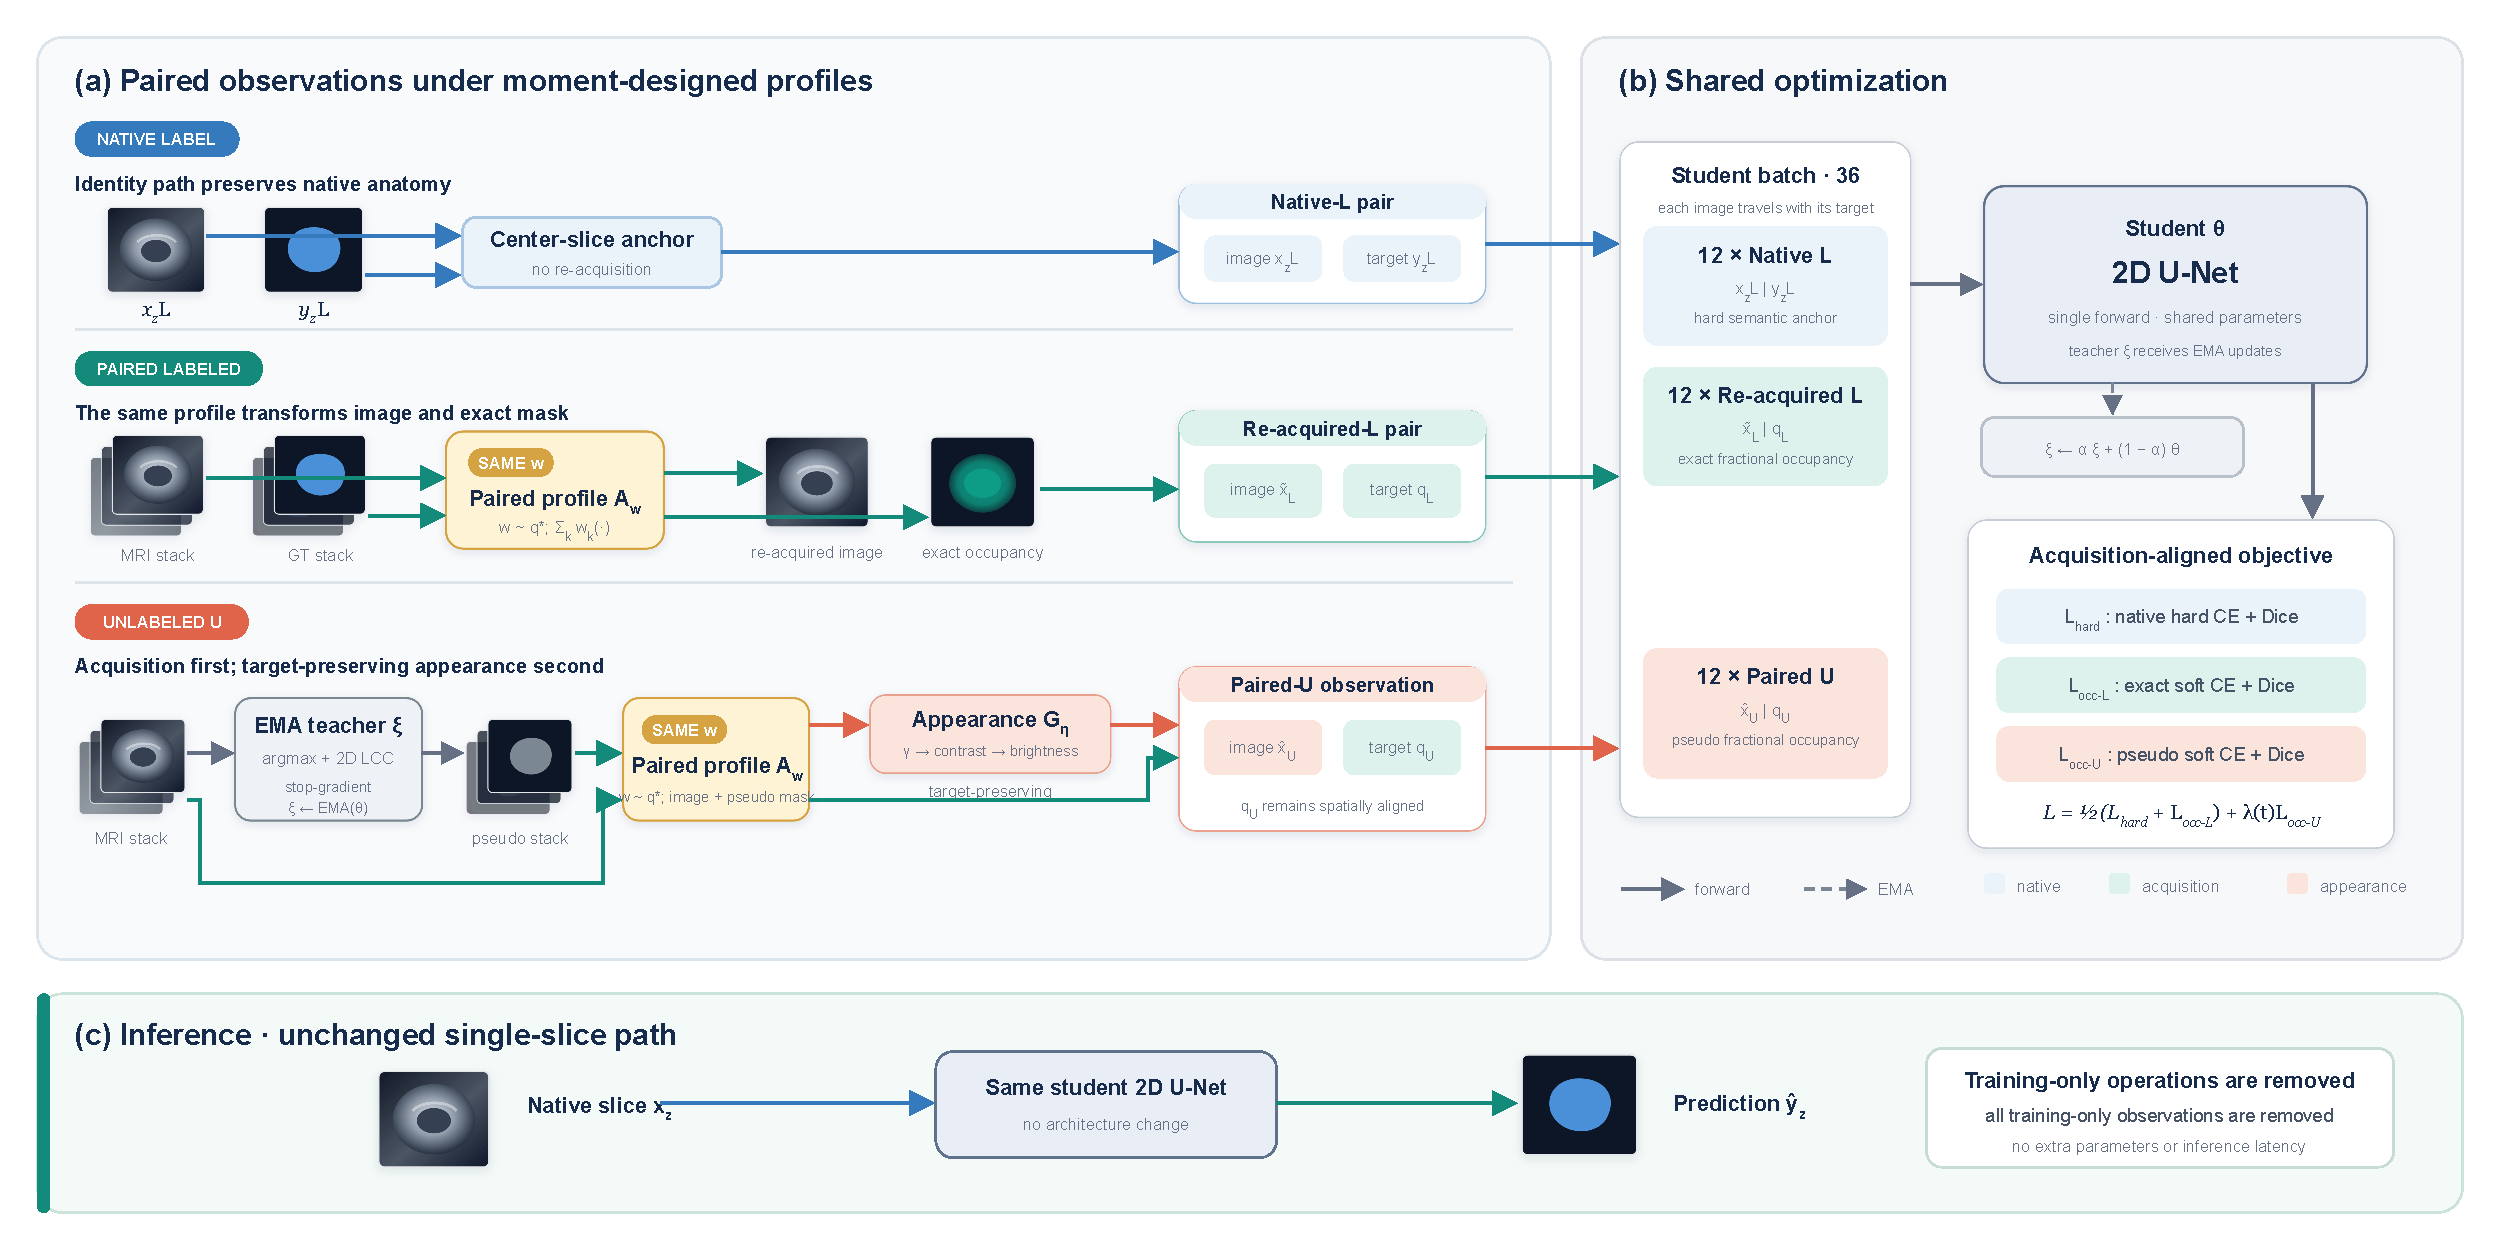
\includegraphics[width=\textwidth]{fig/method_pipeline.pdf}
    \caption{Overview of \method. Native labeled samples provide a hard semantic anchor, while labeled and unlabeled neighboring slices are transformed into paired image--occupancy observations by the same sampled profile. A single student is optimized from all views and updates the EMA teacher. The profile law is designed once from labeled training data, and inference remains an unchanged single-slice 2D path.}
    \label{fig:method}
\end{figure*}

\section{Experiments}

\subsection{Experimental Protocol}
Our experiments answer four questions: (i) does \method{} improve segmentation in low-label regimes; (ii) does the same formulation transfer from prostate to multi-class cardiac MRI; (iii) are paired fractional targets and moment-constrained profile design individually necessary; and (iv) do improvements occur where through-plane partial-volume effects are expected to be strongest?

All methods use identical patient splits, labeled identities, preprocessing, backbone, optimizer, validation cadence, checkpoint selector, and test post-processing. Checkpoints are selected by validation performance only, and each test set is evaluated once after all choices are frozen. For MM-WHS, the profile distribution is recomputed from its labeled training subset using the same support, objective, and constraints as PROMISE12; no validation or test sample is used by the distribution design.

\subsection{Datasets}
\paragraph{PROMISE12.}
PROMISE12 contains multi-center, multi-vendor T2-weighted prostate MRI volumes~\cite{litjens2014promise12}. We use the fixed 35/5/10 patient split recorded in the repository. The primary low-label setting exposes 7 of the 35 training annotations; the 11-label setting evaluates annotation scaling. The remaining training cases are treated as unlabeled. Case lists, slice manifests, and preprocessing hashes are held fixed across methods.

\paragraph{MM-WHS MRI.}
MM-WHS contains clinical 3D cardiac MRI and CT volumes with seven foreground structures~\cite{zhuang2019mmwhs}. We use only MRI. Before training, four of the 20 labeled MRI volumes are locked for validation; four training volumes retain labels and the remaining 12 have labels hidden during optimization. We evaluate myocardium, left/right atria, left/right ventricles, ascending aorta, and pulmonary artery. The exact split manifest is committed before execution.

\subsection{Implementation Details}
All PROMISE12 experiments use a 2D U-Net with $256\times256$ inputs, SGD with learning rate 0.01, momentum 0.9 and weight decay $10^{-4}$, EMA decay 0.99, and a loader batch of 12 labeled plus 12 unlabeled slices. Training comprises 10,000 supervised pretraining iterations and 30,000 self-training iterations, including a 1,000-iteration supervised warm-up. After warm-up, \method{} evaluates 36 student views per step: 12 native labeled, 12 paired labeled, and 12 paired unlabeled views. The fixed coordinate-preserving appearance policy uses log-gamma $\pm0.25$, log-contrast $\pm0.1875$, and brightness relative to intensity span $\pm0.125$. Seed 1337 is used for the primary comparison.

MM-WHS retains the method definition, profile-design constraints, and validation-only checkpoint policy. Only dataset-dependent class count, preprocessing, and patch sampling are changed. We report model parameters, training time, peak GPU memory, and single-volume inference time.

\subsection{Metrics and Statistics}
We report patient-level Dice, Jaccard, 95th-percentile Hausdorff distance (HD95), and average surface distance (ASD). MM-WHS distances use physical spacing and are reported in millimeters; macro averages and all seven per-structure Dice scores are included. Primary comparisons are paired by patient. We report mean, standard deviation, median paired difference, and 95\% percentile-bootstrap confidence intervals with 10,000 resamples. A two-sided Wilcoxon signed-rank test is secondary evidence, with Holm correction for multiple comparisons. Statistical tests are not used for checkpoint selection or method tuning.

\subsection{Comparison on PROMISE12}
Table~\ref{tab:promise_main} compares methods under the same 35/5/10 split and training protocol. Results reported under incompatible partitions or backbones are discussed separately and are not mixed into the matched table.

\begin{table*}[t]
\centering
\caption{PROMISE12 comparison under the fixed 35/5/10 split. Higher Dice/Jaccard and lower HD95/ASD are better. Mean$\pm$SD is computed over patients.}
\label{tab:promise_main}
\resizebox{\textwidth}{!}{%
\begin{tabular}{lcccccccccc}
\toprule
& \multicolumn{4}{c}{7 labeled patients} & \multicolumn{4}{c}{11 labeled patients} & \multicolumn{2}{c}{Protocol} \\
\cmidrule(lr){2-5}\cmidrule(lr){6-9}\cmidrule(lr){10-11}
Method & Dice $\uparrow$ & Jac. $\uparrow$ & HD95 $\downarrow$ & ASD $\downarrow$
& Dice $\uparrow$ & Jac. $\uparrow$ & HD95 $\downarrow$ & ASD $\downarrow$
& Seeds & Test use \\
\midrule
Supervised only & \todoresult{} & \todoresult{} & \todoresult{} & \todoresult{}
& \todoresult{} & \todoresult{} & \todoresult{} & \todoresult{} & 1 & once \\
Mean Teacher~\cite{tarvainen2017mean} & \todoresult{} & \todoresult{} & \todoresult{} & \todoresult{}
& \todoresult{} & \todoresult{} & \todoresult{} & \todoresult{} & 1 & once \\
BCP~\cite{bai2023bcp} & \todoresult{} & \todoresult{} & \todoresult{} & \todoresult{}
& \todoresult{} & \todoresult{} & \todoresult{} & \todoresult{} & 1 & once \\
UniMatch~\cite{yang2023unimatch} & \todoresult{} & \todoresult{} & \todoresult{} & \todoresult{}
& \todoresult{} & \todoresult{} & \todoresult{} & \todoresult{} & 1 & once \\
$\beta$-FFT~\cite{hu2025betafft} & \todoresult{} & \todoresult{} & \todoresult{} & \todoresult{}
& \todoresult{} & \todoresult{} & \todoresult{} & \todoresult{} & 1 & once \\
\midrule
\method{} (ours) & \todoresult{} & \todoresult{} & \todoresult{} & \todoresult{}
& \todoresult{} & \todoresult{} & \todoresult{} & \todoresult{} & 1 (3 opt.) & once \\
\bottomrule
\end{tabular}}
\end{table*}

\subsection{Cross-Organ Evaluation on MM-WHS}
Table~\ref{tab:mmwhs_main} tests whether the same paired observation principle and profile-design procedure transfer from binary prostate segmentation to seven-class whole-heart MRI. The primary endpoint is macro Dice; per-structure results reveal whether gains extend beyond large chambers to myocardium and great vessels.

\begin{table*}[t]
\centering
\caption{MM-WHS MRI results under the frozen 4-labeled/12-unlabeled protocol. Method hyperparameters are transferred unchanged; the profile law is designed using labeled training volumes only.}
\label{tab:mmwhs_main}
\resizebox{\textwidth}{!}{%
\begin{tabular}{lcccccccccc}
\toprule
Method & Avg. Dice $\uparrow$ & Avg. HD95 $\downarrow$ & Myo & LA & LV & RA & RV & AO & PA \\
\midrule
Supervised only & \todoresult{} & \todoresult{} & \todoresult{} & \todoresult{} & \todoresult{} & \todoresult{} & \todoresult{} & \todoresult{} & \todoresult{} \\
Mean Teacher & \todoresult{} & \todoresult{} & \todoresult{} & \todoresult{} & \todoresult{} & \todoresult{} & \todoresult{} & \todoresult{} & \todoresult{} \\
UniMatch & \todoresult{} & \todoresult{} & \todoresult{} & \todoresult{} & \todoresult{} & \todoresult{} & \todoresult{} & \todoresult{} & \todoresult{} \\
Paired profile (uniform) & \todoresult{} & \todoresult{} & \todoresult{} & \todoresult{} & \todoresult{} & \todoresult{} & \todoresult{} & \todoresult{} & \todoresult{} \\
\midrule
\method{} (ours) & \todoresult{} & \todoresult{} & \todoresult{} & \todoresult{} & \todoresult{} & \todoresult{} & \todoresult{} & \todoresult{} & \todoresult{} \\
\bottomrule
\end{tabular}}
\end{table*}

\subsection{Controlled Ablation}
The main ablation isolates the two claims of \method{} without treating implementation choices as independent modules. All four configurations process 36 student views and use the same appearance policy, optimizer, teacher, and validation selector.

\begin{table*}[t]
\centering
\caption{Compact ablation on PROMISE12 with 7 labeled patients. ``Paired target'' denotes the operator-induced fractional occupancy. Every row is matched for student-view count and appearance perturbation.}
\label{tab:ablation}
\begin{tabular}{clcccccc}
\toprule
ID & Configuration & 36 views & Image profile & Paired target & MPD & Dice $\uparrow$ & HD95 $\downarrow$ \\
\midrule
A0 & Compute-matched teacher--student & \cmark & -- & -- & -- & \todoresult{} & \todoresult{} \\
A1 & Image-profile only & \cmark & \cmark & -- & -- & \todoresult{} & \todoresult{} \\
A2 & Paired profile, uniform sampling & \cmark & \cmark & \cmark & -- & \todoresult{} & \todoresult{} \\
A3 & \method{} & \cmark & \cmark & \cmark & \cmark & \todoresult{} & \todoresult{} \\
\bottomrule
\end{tabular}
\end{table*}

The contrast A1--A0 tests whether modifying the observation alone creates the predicted image--target mismatch. A2--A1 tests whether pairing the same profile with a fractional target resolves that mismatch. A3--A2 isolates the contribution of moment-constrained distribution design over the uniform parent law. Hard-target and profile-support sensitivity controls are reserved for the supplement because they refine, rather than define, the central hypothesis.

\subsection{Mechanism and Efficiency Analysis}
We examine performance by normalized axial third and foreground area, with particular attention to apex/base and small-target slices where through-plane composition changes most rapidly. We additionally report non-degenerate occupancy rate, center-slice semantic flip rate, and calibration of predictions against fractional targets. For profile design, we compare worst-stratum utility before and after optimization and report constraint slack, entropy retention, and maximum density ratio. These analyses use frozen predictions and cannot alter the selected checkpoint.

Efficiency is reported as training throughput, peak memory, parameters, FLOPs, and inference latency. Since neighboring slices, the EMA teacher, and profile sampling are removed at test time, the parameter count and inference FLOPs are identical to the underlying 2D network.

\subsection{Optional Independent-Seed Replication}
Subject to compute availability, the final configuration is replicated with seeds 1337, 2024, and 3407 after all choices are frozen. Every run is reported; no seed is replaced or selected post hoc.

\begin{table}[t]
\centering
\caption{Independent-seed replication of the final frozen configuration.}
\label{tab:seeds}
\begin{tabular}{lcccc}
\toprule
Seed & Dice & Jaccard & HD95 & ASD \\
\midrule
1337 & \todoresult{} & \todoresult{} & \todoresult{} & \todoresult{} \\
2024 & \todoresult{} & \todoresult{} & \todoresult{} & \todoresult{} \\
3407 & \todoresult{} & \todoresult{} & \todoresult{} & \todoresult{} \\
\midrule
Mean$\pm$SD & \todoresult{} & \todoresult{} & \todoresult{} & \todoresult{} \\
\bottomrule
\end{tabular}
\end{table}

\section{Conclusion}
We introduced \method, a training-only approach that couples a through-plane MRI observation with its operator-induced fractional target and designs the corresponding profile distribution under robust moment constraints. The method addresses a specific failure of label-invariant augmentation: when the observation changes tissue composition, the target must change with it. Because all additional operations are confined to training, \method preserves the original single-slice 2D architecture, parameter count, and inference cost. Evaluation on prostate and cardiac MRI tests both low-label accuracy and cross-organ transfer under matched protocols.


{
    \small
    \bibliographystyle{ieeenat_fullname}
    \bibliography{main}
}

% WARNING: remove supplementary pages from the main submission PDF.
% \input{sec/X_suppl}

\end{document}
